\question{}
\begin{ابجد}
\item در مدل‌سازی مسئله به صورت \lr{CSP} هر کارمند را یک متغیر و سه شیفت مورد نظر را دامنه متغیرها در نظر می‌گیریم:
\begin{itemize}
    \item \textbf{متغیرها}: سارا ($S$)، نهال ($N$)، پریا ($P$) و زهرا ($Z$)
    \item \textbf{دامنه متغیرها}: $\}$صبح (1)، عصر (2)، شب (3)$\{$
    \item \textbf{محدودیت‌ها}:
          \lr{
              \begin{itemize}
                  \item[$C_{SN}$:] $[(S=N \lor S=3 \lor N=3)] \land [(S \neq N \lor S=N=2)]$
                  \item[$C_{ZS}$:] $(Z \neq S) \land (Z > S)$
                  \item[$C_{ZN}$:] $Z \neq N$
                  \item[$C_{ZP}$:] $Z \neq P$
                  \item[$C_{NP}$:] $N \neq P$
              \end{itemize}
          }

          گراف شرط‌های مسئله به این صورت است:
          \begin{figure}[H]
              \centering
              \vspace{-0.2cm}
              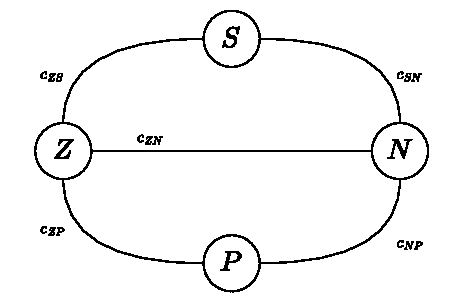
\includegraphics[width=0.5\textwidth]{assets/q3-A-fixed.pdf}
          \end{figure}
\end{itemize}

\item از الگوریتم \lr{AC-3} استفاده می‌کنیم. یک صف (\lr{queue}) از تمام یال‌ها نگه داشته، و در هر مرحله دامنه یک متغیر را با توجه به یال خارج شده به‌روز کرده و در صورت نیاز، یال‌هایی را به صف اضافه می‌کنیم. \\
در هر مرحله یال خارج شده از صف را با رنگ قرمز و یال‌هایی را که در مرحله قبل به صف اضافه شده‌اند (در صورت وجود) را با رنگ آبی نمایش می‌دهیم.

\begin{LTR}
    \begin{longtable}{|c|>{\raggedright\arraybackslash}p{5.5cm}|>{\raggedright\arraybackslash}p{8.0cm}|}
        \hline
        \lr{step} & \lr{Queue}                                                                                                                       & \lr{Domains}                                                                                             \\
        \hline
        \endfirsthead

        \hline
        \lr{step} & \lr{Queue}                                                                                                                       & \lr{Domains}                                                                                             \\
        \hline
        \endhead

        \hline
        \endfoot

        \hline
        \endlastfoot
        1         & \lr{\textcolor{red}{$(S, Z)$}, $(Z, S)$, $(N, S)$, $(S, N)$, $(Z, N)$, $(N, Z)$, $(Z, P)$, $(P, Z)$, $(N, P)$, $(P, N)$}         & \lr{$D(S)=\{1,2,\textcolor{red}{\cancel{3}}\}, D(N)=\{1,2,3\}, \newline D(P)=\{1,2,3\}, D(Z)=\{1,2,3\}$} \\
        \hline

        2         & \lr{\textcolor{red}{$(Z, S)$}, $(N, S)$, $(S, N)$, $(Z, N)$, $(N, Z)$, $(Z, P)$, $(P, Z)$, $(N, P)$, $(P, N)$}                   & \lr{$D(S)=\{1,2\}, D(N)=\{1,2,3\}, \newline D(P)=\{1,2,3\}, D(Z)=\{\textcolor{red}{\cancel{1}},2,3\}$}   \\
        \hline

        3         & \lr{\textcolor{red}{$(N, S)$}, $(S, N)$, $(Z, N)$, $(N, Z)$, $(Z, P)$, $(P, Z)$, $(N, P)$, $(P, N)$, \textcolor{blue}{$(S, Z)$}} & \lr{$D(S)=\{1,2\}, D(N)=\{\textcolor{red}{\cancel{1}},2,3\}, \newline D(P)=\{1,2,3\}, D(Z)=\{2,3\}$}     \\
        \hline

        4         & \lr{\textcolor{red}{$(S, N)$}, $(Z, N)$, $(N, Z)$, $(Z, P)$, $(P, Z)$, $(N, P)$, $(P, N)$, $(S, Z)$}                             & \lr{$D(S)=\{1,2\}, D(N)=\{2,3\}, \newline D(P)=\{1,2,3\}, D(Z)=\{2,3\}$}                                 \\
        \hline

        5         & \lr{\textcolor{red}{$(Z, N)$}, $(N, Z)$, $(Z, P)$, $(P, Z)$, $(N, P)$, $(P, N)$, $(S, Z)$}                                       & \lr{$D(S)=\{1,2\}, D(N)=\{2,3\}, \newline D(P)=\{1,2,3\}, D(Z)=\{2,3\}$}                                 \\
        \hline

        6         & \lr{\textcolor{red}{$(N, Z)$}, $(Z, P)$, $(P, Z)$, $(N, P)$, $(P, N)$, $(S, Z)$}                                                 & \lr{$D(S)=\{1,2\}, D(N)=\{2,3\}, \newline D(P)=\{1,2,3\}, D(Z)=\{2,3\}$}                                 \\
        \hline

        7         & \lr{\textcolor{red}{$(Z, P)$}, $(P, Z)$, $(N, P)$, $(P, N)$, $(S, Z)$}                                                           & \lr{$D(S)=\{1,2\}, D(N)=\{2,3\}, \newline D(P)=\{1,2,3\}, D(Z)=\{2,3\}$}                                 \\
        \hline

        8         & \lr{\textcolor{red}{$(P, Z)$}, $(N, P)$, $(P, N)$, $(S, Z)$}                                                                     & \lr{$D(S)=\{1,2\}, D(N)=\{2,3\}, \newline D(P)=\{1,2,3\}, D(Z)=\{2,3\}$}                                 \\
        \hline

        9         & \lr{\textcolor{red}{$(N, P)$}, $(P, N)$, $(S, Z)$}                                                                               & \lr{$D(S)=\{1,2\}, D(N)=\{2,3\}, \newline D(P)=\{1,2,3\}, D(Z)=\{2,3\}$}                                 \\
        \hline

        10        & \lr{\textcolor{red}{$(P, N)$}, $(S, Z)$}                                                                                         & \lr{$D(S)=\{1,2\}, D(N)=\{2,3\}, \newline D(P)=\{1,2,3\}, D(Z)=\{2,3\}$}                                 \\
        \hline

        11        & \lr{\textcolor{red}{$(S, Z)$}}                                                                                                   & \lr{$D(S)=\{1,2\}, D(N)=\{2,3\}, \newline D(P)=\{1,2,3\}, D(Z)=\{2,3\}$}                                 \\
        \hline

        12        & \lr{$\emptyset$}                                                                                                                 & \lr{$D(S)=\{1,2\}, D(N)=\{2,3\}, \newline D(P)=\{1,2,3\}, D(Z)=\{2,3\}$}                                 \\
        \hline
    \end{longtable}
\end{LTR}

همان طور که مشاهده می‌شود، در انتها دامنه‌ها به این صورت هستند:
\begin{align*}
     & D(S) = \{1, 2\}    \\
     & D(N) = \{2, 3\}    \\
     & D(P) = \{1, 2, 3\} \\
     & D(Z) = \{2, 3\}
\end{align*}

\end{ابجد}